\documentclass[tikz,border=12pt]{standalone}
\usepackage{amsmath,amssymb}
\usetikzlibrary{calc,arrows.meta}

\begin{document}
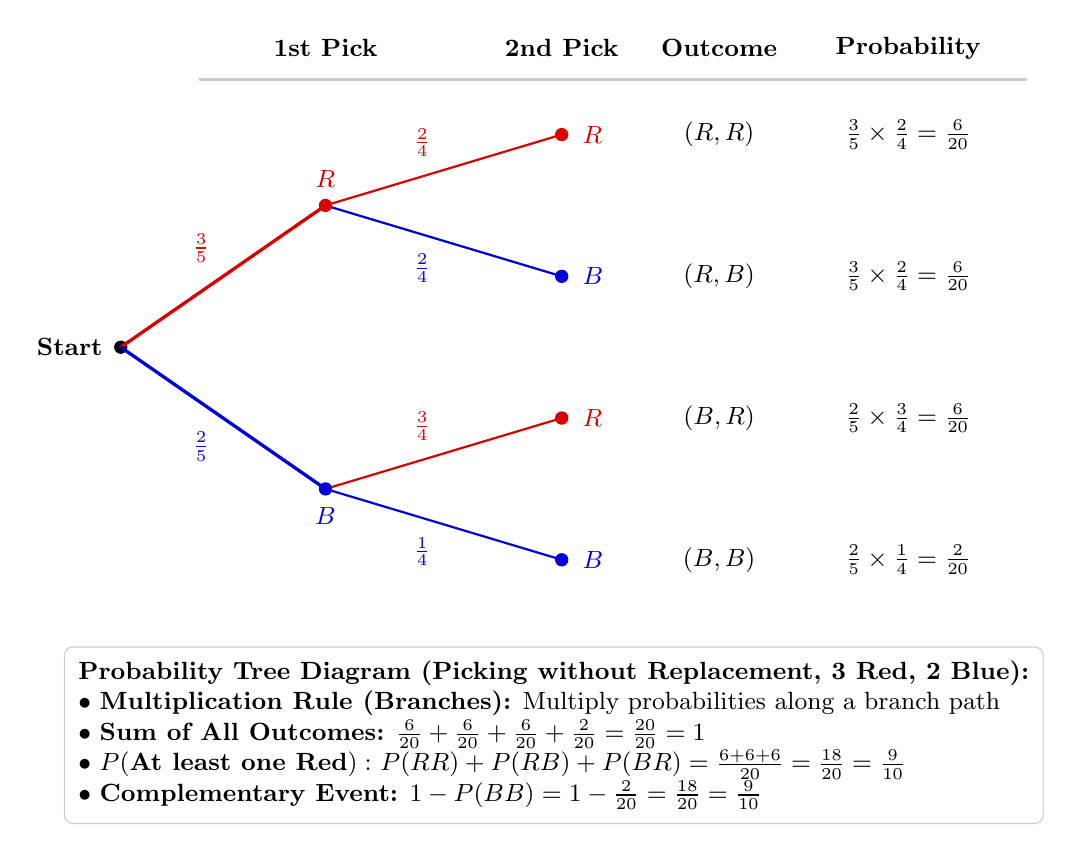
\begin{tikzpicture}[>=latex, line cap=round, line join=round]

  % Column Headers
  \node[font=\small\bfseries] at (2.6, 3.8) {1st Pick};
  \node[font=\small\bfseries] at (5.6, 3.8) {2nd Pick};
  \node[font=\small\bfseries] at (7.6, 3.8) {Outcome};
  \node[font=\small\bfseries] at (10.0, 3.8) {Probability};

  % Dividing guide header line
  \draw[thick, gray!40] (1.0, 3.4) -- (11.5, 3.4);

  % Root
  \coordinate (Root) at (0, 0);
  \filldraw[black] (Root) circle (2.2pt) node[left=3pt, font=\small\bfseries] {Start};

  % Stage 1 Coordinates
  \coordinate (R1) at (2.6, 1.8);
  \coordinate (B1) at (2.6, -1.8);

  % Stage 2 Coordinates
  \coordinate (RR) at (5.6, 2.7);
  \coordinate (RB) at (5.6, 0.9);
  \coordinate (BR) at (5.6, -0.9);
  \coordinate (BB) at (5.6, -2.7);

  % Stage 1 Branches
  \draw[very thick, red!85!black] (Root) -- (R1) node[midway, above left=1pt, font=\small\bfseries] {$\frac{3}{5}$};
  \draw[very thick, blue!85!black] (Root) -- (B1) node[midway, below left=1pt, font=\small\bfseries] {$\frac{2}{5}$};

  % Stage 2 Branches from R1
  \draw[thick, red!85!black] (R1) -- (RR) node[midway, above left=1pt, font=\footnotesize\bfseries] {$\frac{2}{4}$};
  \draw[thick, blue!85!black] (R1) -- (RB) node[midway, below left=1pt, font=\footnotesize\bfseries] {$\frac{2}{4}$};

  % Stage 2 Branches from B1
  \draw[thick, red!85!black] (B1) -- (BR) node[midway, above left=1pt, font=\footnotesize\bfseries] {$\frac{3}{4}$};
  \draw[thick, blue!85!black] (B1) -- (BB) node[midway, below left=1pt, font=\footnotesize\bfseries] {$\frac{1}{4}$};

  % Node circles and labels
  % Stage 1 (placed above/below vertex to clear departing branches)
  \filldraw[red!85!black] (R1) circle (2.2pt) node[above=3pt, font=\small\bfseries] {$R$};
  \filldraw[blue!85!black] (B1) circle (2.2pt) node[below=3pt, font=\small\bfseries] {$B$};

  % Stage 2
  \filldraw[red!85!black] (RR) circle (2.2pt) node[right=4pt, font=\small\bfseries] {$R$};
  \filldraw[blue!85!black] (RB) circle (2.2pt) node[right=4pt, font=\small\bfseries] {$B$};
  \filldraw[red!85!black] (BR) circle (2.2pt) node[right=4pt, font=\small\bfseries] {$R$};
  \filldraw[blue!85!black] (BB) circle (2.2pt) node[right=4pt, font=\small\bfseries] {$B$};

  % Outcomes & Probabilities
  \node[font=\small\bfseries] at (7.6, 2.7) {$(R, R)$};
  \node[font=\small] at (10.0, 2.7) {$\frac{3}{5} \times \frac{2}{4} = \frac{6}{20}$};

  \node[font=\small\bfseries] at (7.6, 0.9) {$(R, B)$};
  \node[font=\small] at (10.0, 0.9) {$\frac{3}{5} \times \frac{2}{4} = \frac{6}{20}$};

  \node[font=\small\bfseries] at (7.6, -0.9) {$(B, R)$};
  \node[font=\small] at (10.0, -0.9) {$\frac{2}{5} \times \frac{3}{4} = \frac{6}{20}$};

  \node[font=\small\bfseries] at (7.6, -2.7) {$(B, B)$};
  \node[font=\small] at (10.0, -2.7) {$\frac{2}{5} \times \frac{1}{4} = \frac{2}{20}$};

  % Summary Card below
  \node[align=left, font=\small, fill=white, inner sep=5pt, draw=gray!40, rounded corners=3pt, anchor=north] at (5.5, -3.8) {
    \textbf{Probability Tree Diagram (Picking without Replacement, 3 Red, 2 Blue):}\\
    $\bullet$ \textbf{Multiplication Rule (Branches):} Multiply probabilities along a branch path\\
    $\bullet$ \textbf{Sum of All Outcomes:} $\frac{6}{20} + \frac{6}{20} + \frac{6}{20} + \frac{2}{20} = \frac{20}{20} = 1$\\
    $\bullet$ \textbf{$P(\text{At least one Red}):$} $P(RR) + P(RB) + P(BR) = \frac{6 + 6 + 6}{20} = \frac{18}{20} = \frac{9}{10}$\\
    $\bullet$ \textbf{Complementary Event:} $1 - P(BB) = 1 - \frac{2}{20} = \frac{18}{20} = \frac{9}{10}$
  };

\end{tikzpicture}
\end{document}
